\documentclass[11pt]{article}
\usepackage{amsmath}
% use UTF8 encoding
\usepackage[utf8]{inputenc}
% use KoTeX package for Korean
\usepackage{kotex}

\usepackage{hyperref}

\usepackage{graphicx}

\hypersetup{
    colorlinks=true,   
    urlcolor=red,
}

\title{정원 관리를 위한 스마트 플랫폼 개발}

\author{Minwoo Jung}

\begin{document}
\maketitle
\indent \\스마트팜 플랫폼은 엣지계층과 서버계층으로 구분한다. 엣지계층은 토양센서모듈과 데이터융합모듈을 포함하고 있다.
토양센서모듈(End device)은 토양센서와 센서제어모듈로 구성한다. 토양센서는 토양정보를 실시간으로 센싱할 수 있다. 
대표적인 토양센서는 온습도센서, NPK센서, PH센서, EC센서 등이 있다.

\indent \\센서제어모듈은 토양센서를 통해 입력된 토양정보를 기반으로 워터펌프를 제어할 수 있는 closed-loop system이다. 센서제어모듈의 기능은 RS-485통신 기반 다중센서제어, 정밀한 액츄에어터제어, 원격통신을 위한 다양한 무선통신(BLE, WiFi, LoRa) 지원한다. 센서제어모듈은 토양센서를 다중연결하기 위해서 RS-485 통신을 사용하였다. RS-485 통신은 시리얼통신 방식이다. 시리얼통신의 데이터 전송방식은 전이중(Full duplex)방식과 반이중(Half duplex) 방식으로 구분된다. 전이중방식은 데이터 송수신을 동시에 할 수 있는 방식이다. 전이중방식의 대표적인 예는 휴대전화이다. 반이중방식은 데이터 송수신을 동시에 할 수 없는 방식이다. 반이중방식의 대표적인 예는 무전기이다. RS-485은 반이중방식으로 데이터를 송수신한다. 데이터 전송거리가 다른 통신방식보다 길다는 장점을 가진다. 최대 통달거리는 1.2 km에 달한다. 전송거리는 전송속도와 상관관계를 가진다. RS-485는 전송속도 100kbps에서 통달거리 1.2km까지 가능하고, 전송속도 10Mbps에서 통달거리는 12m로 감소한다. RS-485는 다중 장비들의 네트워크 생성이 가능한 멀티드롭(Multi-Drop) 방식이다. 멀티드롭 방식은 멀티포인트 방식이라고도 일컬어지며, 다중 장비를 하나의 회선에 연결하는 방식이다. 멀티드롭에 사용하는 장비는 주소판단기능과 데이터 블록을 일시적으로 저장할 수 있는 버퍼 기억장치를 가지고 있어야한다. 데이터 양과 회서 점유시간이 적을 떄 매우 효율적이다. 

\indent \\토양센서는 JXCT사 JXBS 시리즈를 사용한다. 토양센서는 온습도센서, NPK센서, PH센서, EC센서를 활용한다. 토양센서는 RS-485 기반 Modbus-RTU 통신프로토콜을 지원한다. Modbus-RTU 프로토콜은 마스터/슬레이브 기반 아키텍처로 RS-485 통신을 지원한다. Modbus-RTU 프로토콜의 주요 목적은 자동화와 필드 기기 간 빠르고 안정적인 통신이 가능하다. Modbus-RTU는 정해진 메모리맵을 지원하기 떄문에 장비가 바뀌어도 프로토콜은 바뀌지 않는다. 토양센서는 지정된 레지스터 주소에 접근하여 읽기/쓰기가 가능하다. 송수신 메시지 구조(Message frame)는 모든 센서가 동일하다. 기본적인 데이터 구조는 그림 \ref{Data_Frame}과 같다. Address Code는 센서 식별코드로 버스 상에 다중으로 연결된 센서를 구분하기 위한 기능이다. Function Code는 동작을 정의하기 위한 코드로 읽기(0x03/0x04)와 쓰기(0x06) 기능을 포함하고 있다.
Register start address는 접근하기 위한 레지스터의 시작주소를 나타내며, Register length는 데이터를 포함한 길이이다. 

\indent \\본 연구에서 솔레노이드 밸브를 제어하기 위해서 12V 릴레이(sla-12vdc-sl-a)를 활용하였다. 릴레이는 개폐장치(연결/비연결) 기능을 가지는 소자이다. 환경센서정보를 기반으로 솔레노이드 밸브를 정밀하게 제어할 수 있는 Closed loop 환경을 구축한다. 

\indent \\스마트팜에서 가장 중요한 부분은 적절한 토양 선정과 정확한 관수 주기 조절이다. 토양은 일반적으로 질토, 양토, 사토로 나눌 수 있다.
질토는 진흙으로만 이루어진 토양을 말하며, 흙의 입자가 조밀하고 부드러워 지력이 좋다. 작물 성장 입장에서는 튼실하게 자라지만, 성장이 느리다. 수분 저장력이 높아서 가뭄에 강하다. 유기물의 저장력이 좋아서 초기 생장은 느리지만 점차 성장속도가 빨라진다.
양토는 흙의 입자가 질토와 사토 중간 형태의 적당한 크기이다. 지력이 보통이하로 좋지 않아 작물 생장속도는 평균 이하이다. 수분이나 유기물 저장력 또한 평균적이어서 초기 생육은 좋지만, 점점 생장속도가 저하된다.
사토는 흙의 입자가 굵고 거칠어서 지력과 저장력이 좋지 않다. 초기 생장은 아주 좋지만, 결실을 맺기 어렵다. 


\begin{figure}[!htbp]
    \centering
       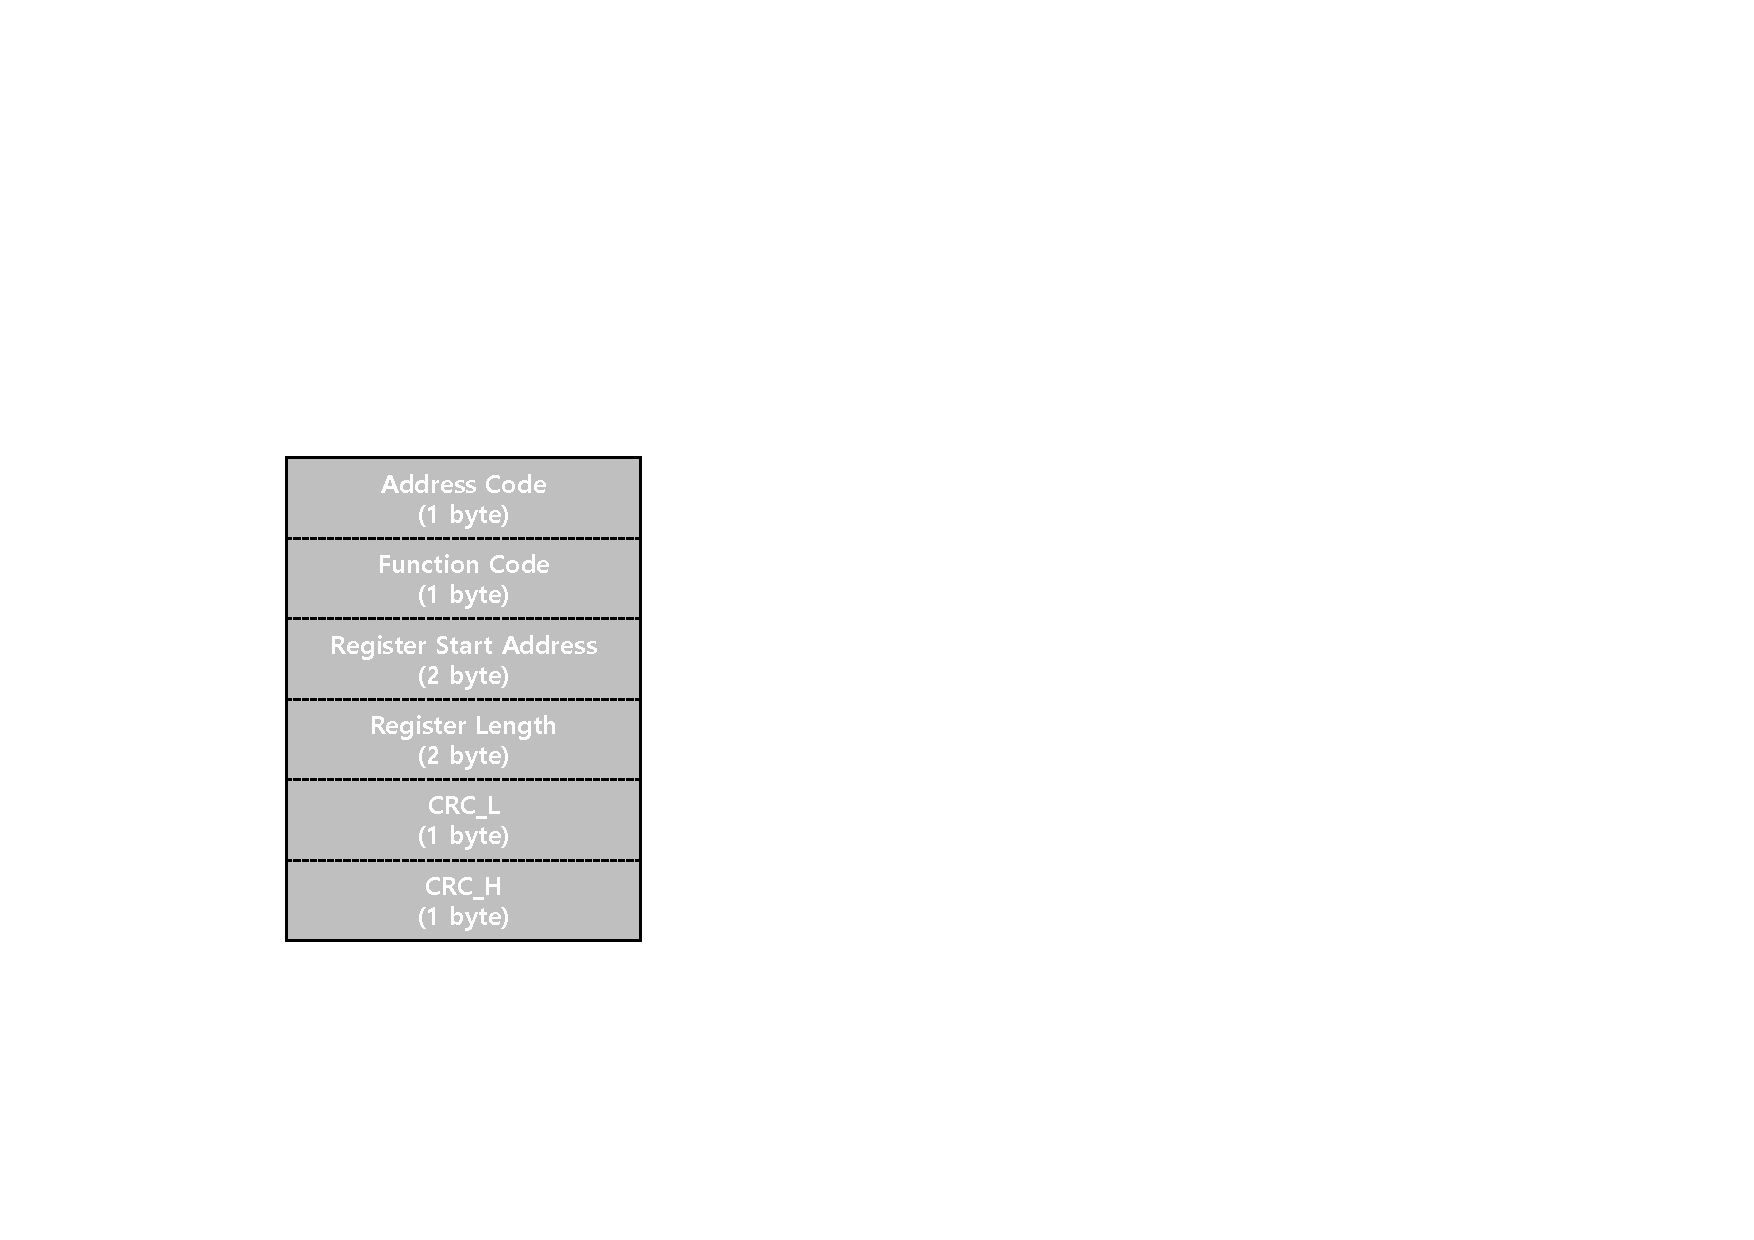
\includegraphics[width=8.5cm]{Figure/Frame_format.pdf}
       \hfil
    \caption{Data Frame}
    \label{Data_Frame}
\end{figure}

토양센서


\indent \\

\end{document}